\documentclass{sig-alternate-05-2015}

\usepackage[utf8]{inputenc}
\usepackage{amsmath}
\usepackage{xparse}

\usepackage[dvipsnames]{xcolor} % color names
\usepackage{moresize} % give more size options than the standard ones
\usepackage{hyperref}
\usepackage[inline]{enumitem}
\usepackage{seqsplit}
\usepackage[british]{babel}


\usepackage{listings}
\lstset{
	tabsize=1,
	frame=lines,
	%caption=sample caption,
	captionpos=b,
	%abovecaptionskip=10pt,
	%belowcaptionskip=10pt,
	%label=code:sample,
	frame=shadowbox,
	rulesepcolor=\color{gray},
	xleftmargin=10pt,
	%framexleftmargin=15pt,
	identifierstyle=\color{Brown}\ttfamily,
	%keywordstyle=\color{Green}\bf\ttfamily,
	commentstyle=\color{OliveGreen},
	stringstyle=\color{Brown}\ttfamily,
	numbers=left,
	numberstyle=\tiny,
	numbersep=5pt,
	%breaklines=true,
	showstringspaces=false,
	basicstyle=\fontsize{9}{9}\ttfamily, %\tiny,  %\footnotesize\ttfamily,  % or e.g., \ssmal to get small font in listings
	morecomment=[n]{/*}{*/},
	morekeywords={},
	breaklines=true,
	postbreak=\raisebox{0ex}[0ex][0ex]{\ensuremath{\color{red}\hookrightarrow\space}}
	emph={for,each,if,else,then,in,is,create,IN
	},emphstyle={\color{blue}\bf\ttfamily}
}

\newcommand{\erestr}[2]{\exists\;\,{\tt #1}\,.\,{\tt #2}}
\DeclareDocumentCommand\node{ m g }{{\tt #1\IfNoValueF {#2} {{:}#2}}}



\begin{document}

% Copyright
\setcopyright{acmcopyright}
%\setcopyright{acmlicensed}
%\setcopyright{rightsretained}
%\setcopyright{usgov}
%\setcopyright{usgovmixed}
%\setcopyright{cagov}
%\setcopyright{cagovmixed}


% DOI
\doi{DOI}

% ISBN
\isbn{ISBN}

%Conference
\conferenceinfo{SEMANTICS '17}{September 16--19, 2017, Amsterdam, The Netherlands}

\acmPrice{\$0.00}

%
% --- Author Metadata here ---

\conferenceinfo{SEMANTICS}{'2017 Amsterdam, The Netherlands}

% --- End of Author Metadata ---

\title{Towards IoT platforms' integration: Semantic Translations between \ttlit{W3C SSN} and \ttlit{ETSI SAREF}}
%\title{Alternate {\ttlit ACM} SIG Proceedings Paper in LaTeX
%Format\titlenote{(Produces the permission block, and
%copyright information). For use with
%SIG-ALTERNATE.CLS. Supported by ACM.}}
%\subtitle{[Extended Abstract]
%\titlenote{A full version of this paper is available as
%\textit{Author's Guide to Preparing ACM SIG Proceedings Using
%\LaTeX$2_\epsilon$\ and BibTeX} at
%\texttt{www.acm.org/eaddress.htm}}}

\numberofauthors{9} %  in this sample file, there are a *total*

\author{
% You can go ahead and credit any number of authors here,
% e.g. one 'row of three' or two rows (consisting of one row of three
% and a second row of one, two or three).
%
% The command \alignauthor (no curly braces needed) should
% precede each author name, affiliation/snail-mail address and
% e-mail address. Additionally, tag each line of
% affiliation/address with \affaddr, and tag the
% e-mail address with \email.
%
% 1st. author
\alignauthor
%ABC\thanks{XYZ} \and DEF\thanks{UVW} \and GHI\footnotemark[1]
João Moreira\thanks{University of Twente, Enschede, The Netherlands.\newline\{j.luizrebelomoreira@utwente.nl, l.ferreirapires@utwente.nl, m.j.vansinderen\}@utwente.nl} 
%       \affaddr{University of Twente}\\
%       \affaddr{Enschede, The Netherlands}\\
%       \email{j.luizrebelomoreira@utwente.nl}
% 2nd. author
\alignauthor
Laura Daniele\thanks{Netherlands Organisation for Applied Scientific Research, TNO.\newline laura.daniele@tno.nl}\\
%       \affaddr{TNO}\\
%       \affaddr{The Haugue, The Netherlands}\\
%       \email{Laura.Daniele@tno.nl}
% 3rd. author
\alignauthor 
Luis Ferreira Pires\footnotemark[1]\\
%       \affaddr{University of Twente}\\
%       \affaddr{Enschede, The Netherlands}\\
%       \email{larst@affiliation.org}
\and  % use '\and' if you need 'another row' of author names
% 4th. author
\alignauthor 
Marten van Sinderen\footnotemark[1]\\
%       \affaddr{University of Twente}\\
%       \affaddr{Enschede, The Netherlands}\\
%       \email{lleipuner@researchlabs.org}
% 5th. author
\alignauthor 
Katarzyna Wasielewska\thanks{Systems Research Institute, Polish Academy of Sciences, Warsaw, Poland \newline\{katarzyna.wasielewska, pawel.szmeja, maria.ganzha, marcin.paprzycki\}@ibspan.waw.pl}\\
%       \affaddr{Systems Research Institute, Polish Academy of Sciences}\\
%       \affaddr{Warsaw, Poland}\\
%       \email{katarzyna.wasielewsk@ibspan.waw.pl}
% 6th. author
\alignauthor 
Pawel Szmeja\footnotemark[3]\\
%       \affaddr{Systems Research Institute, Polish Academy of Sciences}\\
%       \affaddr{Warsaw, Poland}\\
%       \email{fogartys@amesres.org}
\and  % use '\and' if you need 'another row' of author names
% 7th. author
\alignauthor 
Wiesław Pawłowski\thanks{Faculty of Mathematics, Physics, and Informatics, University of Gdańsk, Poland\newline w.pawlowski@inf.ug.edu.pl}\\
%       \affaddr{Systems Research Institute, Polish Academy of Sciences}\\
%       \affaddr{Warsaw, Poland}\\
%       \email{lleipuner@researchlabs.org}
% 8th. author
\alignauthor 
Maria Ganzha\footnotemark[3]\\
%       \affaddr{Systems Research Institute, Polish Academy of Sciences}\\
%       \affaddr{Warsaw, Poland}\\
%       \email{fogartys@amesres.org}
% 9th. author
\alignauthor 
Marcin Paprzycki\footnotemark[3]\\
%       \affaddr{Systems Research Institute, Polish Academy of Sciences}\\
%       \affaddr{Warsaw, Poland}\\
%       \email{fogartys@amesres.org}
}
% There's nothing stopping you putting the seventh, eighth, etc.
% author on the opening page (as the 'third row') but we ask,
% for aesthetic reasons that you place these 'additional authors'
% in the \additional authors block, viz.
%\additionalauthors{Additional authors: John Smith (The Th{\o}rv{\"a}ld Group,
%email: {\texttt{jsmith@affiliation.org}}) and Julius P.~Kumquat
%(The Kumquat Consortium, email: {\texttt{jpkumquat@consortium.net}}).}
%\date{30 July 1999}
% Just remember to make sure that the TOTAL number of authors
% is the number that will appear on the first page PLUS the
% number that will appear in the \additionalauthors section.

\maketitle
\begin{abstract}
Several IoT ontologies have been developed lately to improve the semantic interoperability of IoT solutions. The most popular ontology, the W3C Semantic Sensor Network (SSN), is considered an ontological foundation for diverse IoT initiatives, as OpenIoT. With characteristics similar to SSN, the ETSI Smart Appliances REFerence (SAREF) ontology evolved from the needs of smart home solutions to common requirements of IoT. Some IoT solutions rely on platform-specific ontologies and their integration requires mechanisms to align these ontologies. 
In this paper we discuss the ontology alignments between SSN and SAREF, identifying mapping alternatives and proposing basic mappings that can be re-used to define complex ones. We introduce here an initial specification of the semantic translations from the main elements of SSN to SAREF, which includes classes, object properties and data properties. The alignments will be used in a semantic matching process leveraging the semantic mediator component of the INTER-IoT project. An initial evaluation of the translation was executed by translating the wind sensor (Vaisala WM30), an example provided by the W3C, from SSN to SAREF. This initial evaluation demonstrates the proposal's coherence and feasibility.
\end{abstract}


%
% The code below should be generated by the tool at
% http://dl.acm.org/ccs.cfm
% Please copy and paste the code instead of the example below. 
%
\begin{CCSXML}
<ccs2012>
<concept>
<concept_id>10002951.10003260.10003309.10003315</concept_id>
<concept_desc>Information systems~Semantic web description languages</concept_desc>
<concept_significance>500</concept_significance>
</concept>
</ccs2012>
\end{CCSXML}

\ccsdesc[500]{Information systems~Semantic web description languages}


%
% End generated code
%

%
%  Use this command to print the description
%
\printccsdesc

% We no longer use \terms command
%\terms{Theory}

\keywords{Semantic interoperability, internet-of-things, ontology alignment, SAREF, W3C SSN}

\section{Introduction}

Over the past few years, numerous IoT ontologies were proposed to improve the semantic interoperability of IoT artifacts, i.e. the common understanding capabilities of platforms, devices, gateways, applications and networks involved in IoT solutions \cite{Ganzha2016a}. In this context, the W3C Semantic Sensor Network (SSN) is considered an ontological foundation for the IoT, covering the application of diverse types of sensors, widely used by initiatives as OpenIoT \cite{Soldatos2015} and INTER-IoT \cite{Ganzha2017a}. 
Recently, the Smart Appliances REFerence (SAREF) ontology has evolved from the smart appliances domain (e.g. smart ovens and refrigerators) \cite{Daniele2015} to cover other characteristics of the IoT domain \cite{Daniele2016b}, being created in close interaction with the smart home market \cite{Daniele2016}. It is grounded on 47 “semantic assets”, i.e. standards, proprietary data models, protocols and other ontologies, as SSN. 

IoT platforms enable software engineers to bridge the gap between device sensors and connected applications through suites of components, which can include semantic technologies, e.g. FIWARE with the Sense2Web linked-data generic enabler (GE) and OpenIoT with its own ontology extended from SSN. The Inter-IoT project\footnote{\url{www.inter-iot-project.eu}} aims at design, implement and experiment voluntary interoperability among heterogeneous IoT platforms. The project is driven by use cases from (e/m)Health and transportation / logistics at the port of Valencia, which require semantic integration among IoT artifacts relying on SSN and SAREF.  

A challenge to enable semantic integration between IoT artifacts relying on SSN and SAREF, is how to semantic translate from an one ontology to another, i.e. align these ontologies. To deal with this problem, the development of ontology alignments between SSN and SAREF is required, i.e. finding and mapping the correspondences between entities (atomic) or groups of entities and sub-structures (complex). An approach to implement ontology alignment is semantics translation, which is a process that transforms some information described semantically, in terms of a source ontology, to information described in terms of a target ontology \cite{Ganzha2015}. 

In this paper we describe the initial unidirectional mappings from SSN to SAREF towards their bi-directional semantic translations. We adopted a software engineering methodology including specification and implementation to develop these semantic translations. Here we described the mappings among the main elements for the semantic translations from SSN 1.0 to SAREF 2.0. This specification will be used for further configuration and deployment in the Inter-Platform Semantic Mediator (IPSM) of the INTER-IoT project. An evaluation of these initial mappings is presented, demonstrating how the SSN description of the WM30 wind sensor, an example provided by the W3C, is translated from SSN to SAREF. The semantics of the generated ontology are verified, whether was maintained or lost after the execution of the translations. 

Section 2 describes the background research, including an overview of the IPSM architecture, the SSN and SAREF ontologies. Section 3 describes the methodology used to develop the semantic translations. Section 4 introduces the mappings from SSN to SAREF, describes the evaluation of the mappings and discusses the challenges. Section 5 concludes this work by presenting the lessons learned and future work. 

%%%%%%%%%%%%%%%%%%% SEC: BACKGROUND %%%%%%%%%%%%%%%%%%% 

\section{BACKGROUND}

\subsection{INTER-IoT semantic mediator}
The H2020 project Interoperability of Heterogeneous IoT Platforms (INTER-IoT) \cite{Ganzha2016,Ganzha2017a} main goal is to design,  implement and validate a framework that will allow interoperability between heterogeneous IoT platforms across the transportation / logistics and (e/m)Health appliances domains. The use case scenarios are based on real world situations that need integration among IoT platforms, as the port authority IoT platform, the haulier IoT platform, systems as the container terminal system, port management system and the emergency incidents system. The (e/m)Health domain scenarios aims at improving interoperability among IoT artifacts for patient monitoring, e.g. body sensor networks, wearable and non-wearable devices. Some of these IoT artifacts rely on SSN, such as the OpenIoT platform. In the scenario of detecting emergencies at the port by monitoring drivers' vital signs with medical wearable devices, semantic translations are required between these SSN-based IoT artifacts and smart appliances based on SAREF, e.g. building sensors for vehicle collision detection, security and electrical systems.

INTER-IoT is currently developing the  Inter-Platform Semantic Mediator (IPSM) tool. IPSM is a software tool that follows the semantic interoperability design patterns identified in INTER-IoT, and is intended to be used as part of the translation process defined in the methodology (INTER-Meth). The process of achieving semantic interoperability involves the following steps:

\begin{enumerate*}[label=\roman*)]
	\item lift semantics to a common format and make it explicit \cite{Ganzha2017a}
	\item develop, or choose, a central modular ontology
	\item prepare uni-directional alignments between ontologies of communicating artifacts and the central ontology
	\item establish a multi-channel (1-1, 1-many, many-1) communication architecture that will facilitate translations in all needed contexts, with the central ontology as intermediary
\end{enumerate*}

%The following tasks are executed as part of the IPSM design and implementation to:  (2) develop a central modular ontology, consisting of a core IoT ontology and domain specific modules, (3) preparealignments between ontologies of communicating artefacts and the central ontology,  (4) use the alignments for translations, and (5) establish a multi-channel (1-1, 1-many, many-1) communication architecture that will facilitate translations in all needed contexts.

INTER-IoT provides its own alignment format~\cite{Pawlowski2017}, based on alignment API, to represent interconnections between semantic data with a given ontology. IPSM utilizes alignment files and provides a multi-channel environment for any willing artifact. Pairs of uni-directional alignments between the central ontology and artifact ontology are used to translate messages to and from the central ontology. This enables connection of new artifacts without upsetting existing channels, and requires each participant to provide only a pair of alignments.

\begin{figure}[h!]
\centering
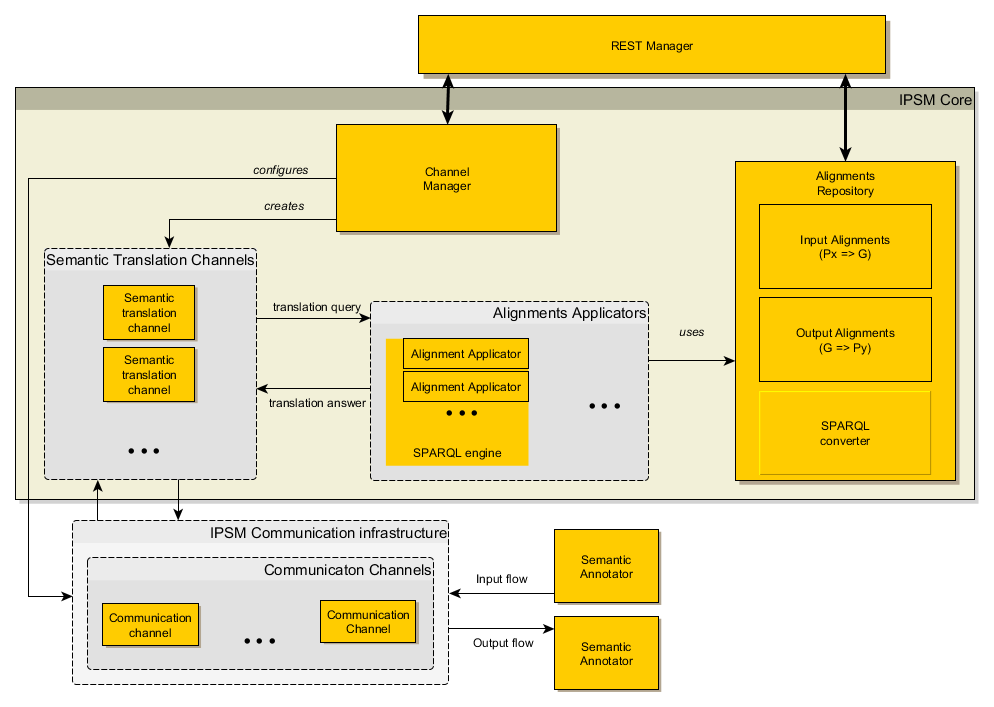
\includegraphics[scale=0.22]{IPSM}
\caption{Inter-Platform Semantic Mediator}
\label{fig:IPSM}
\end{figure}

While complete ontologies are used to build semantic understanding, only conversation-specific alignments are stored and used for actual translations. Figure \ref{fig:IPSM} illustrates IPSM architecture. Ontology alignments and translation channels can be managed through the REST Manager.

\subsection{W3C Semantic Sensor Network (SSN)}
The W3C Semantic Sensor Network (SSN) \cite{Compton2012} is an ontology developed by W3C (last version published in 2011 in the official URL \url{https://www.w3.org/2005/Incubator/ssn/ssnx/ssn}). It provides a comprehensive framework to describe sensors, devices, observations, measurements and other related concepts, enabling reasoning of individual sensors and the connection of a set of sensors, such as a wireless network. SSN is grounded in a set of existing ontologies and standards, such as CSIRO, SWAMO, MMI Device, SEEK Extensible Observation, SemSOS and OGC SensorML \cite{Ganzha2016a}. The main concept of SSN is the \textit{Sensing Device}, which is a sensor that reports measurements and observations of real world phenomena. A sensor is different in nature from other types of devices, e.g. actuators, because of its event-based behavior, which requires temporal relationships. SSN enables reasoning, which can ease the development of advanced applications, for example, by reasoning about sensor measurements, considering constraints as power restriction and limited memory. 

The SSN ontology is composed of 10 modules (Deployment, System, OperatingRestriction, PlatformSite, Device, Process, Data, SSOPlatform, MeasuringCapability, Constra intBlock), representing 41 concepts and 39 object properties. It inherits 11 concepts and 14 object properties from the foundational ontology DOLCE-UltraLite (DUL) (http://ont ologydesignpatterns.org/wiki/Ontology:DOLCE+DnS\_Ultra lite). In this paper we cover the following modules:
\\\\\textbf{DUL module:} represents the foundational categorization of \textit{Designed Artifact}, \textit{Method}, \textit{Physical Object}, \textit{Quality}, \textit{Region} and \textit{Situation}. For example, a \textit{Sensing Device} (Measuring module) is a \textit{Designed Artifact} and a \textit{Physical Object}, which observes a \textit{Property} (Skeleton module). A \textit{Property} is an observable \textit{Quality} of an \textit{Event} or \textit{Object}, i.e. "an aspect of an entity that is intrinsic to and cannot exist without the entity and is observable by a sensor". 
\\\\\textbf{Skeleton module:} represents the most basic concepts regarding sensors, as \textit{Sensor}, \textit{Sensing}, \textit{Property} and  \textit{Observation}. A \textit{Sensor} may be a physical device implementing \textit{Sensing}, i.e. it has a sensing method observing some \textit{Property}. "\textit{Sensing} is a process that results in the estimation, or calculation, of the value of a phenomenon". 
\\\\\textbf{Measuring module:} covers the elements \textit{Sensing Device} and \textit{Sensor DataSheet}. As explained above, the first is the main element of SSN. The former represents the data sheet specifications of a sensor. Usually, the properties of a sensor are recorded directly with \textit{hasMeasurementCapability} property of a \textit{Sensor}.
\\\\\textbf{System module:} represents the \textit{System} concept as a \textit{Physical Object} (DUL) composed by other systems (\textit{hasSubSystem}), which has deployment(s) (\textit{hasDeployment}), normal operating environment(s) (\textit{hasOperatingRange}), survival range(s) (\textit{hasSurvivalRange}) and location(s) relative to other entities (\textit{onPlatform}).
\\\\\textbf{Measuring Capability module:} represents the properties and capabilities of measurements, covering the elements \textit{Accuracy}, \textit{Measurement Capability}, \textit{Measurement Property}, among other classes, as well as fundamental object properties as \textit{hasMeasurementCapability} and \textit{hasMeasurementProperty}. \textit{Measurement Capability} and \textit{Measurement Property} are core concepts in SSN, where the first represents a characteristic of a sensor's observations or ability to make observations (e.g. accuracy and range), while the former represents the collection of measurement properties and environmental conditions in which those properties hold, i.e. the specification of a sensor's capabilities. 
\\\\\textbf{Device module:} covers the element \textit{Device}, which is a physical piece of technology (a "system in a box") and can be composed of other (smaller) devices and software components.\\
 
The W3C SSN Incubator Group created an example of the use of SSN by describing the \textbf{Vaisala WM30 wind sensor}\footnote{\url{www.w3.org/2005/Incubator/ssn/ssnx/meteo}}. It describes the measurement capabilities, power supply and operating and survival properties based on the technical specification about the measurement of wind direction and speed, illustrated in Figure \ref{fig:WM30specifications}. This example was initially reported in \cite{Compton2009}, which gives a precise description of the WM30 sensor. However, the axioms representing its main definitions and restrictions are different, following the changes in the TBox of SSN over the past years. Bellow we update these main definitions:
\begin{align*}
  \begin{aligned}
	&\node{WM30}{Vaisala\-\_WM30} \sqsubseteq \node{ssn}{SensingDevice}\\
	&\node{WM30}{Vaisala\-\_WM30} \sqsubseteq\\
	&\qquad\erestr{\node{ssn}{hasSubSystem}}{\node{WM30}{WM30\-\_Wind\-Direction}}\\
	&\node{WM30}{Vaisala\-\_WM30} \sqsubseteq\\
	&\qquad\erestr{\node{ssn}{hasSubSystem}}{\node{WM30}{WM30\-\_WindSpeed}}\\	
	&\node{WM30}{Vaisala\-\_WM30} \sqsubseteq\\
	&\qquad\erestr{\node{ssn}{observes}}{\node{WM30}{\_WindDirection}}\\
	&\node{WM30}{Vaisala\-\_WM30} \sqsubseteq\\
	&\qquad\erestr{\node{ssn}{observes}}{\node{WM30}{\_WindSpeed}}\\
  \end{aligned}\\
\end{align*}

These axioms represent the Vaisala WM30 as a \textit{Sensing Device} (therefore a \textit{Device} (\textit{System}) and a \textit{Sensor}), composed by (\textit{hasSubSystem}) WM30 particular sensors for wind direction and wind speed, being able to measure (\textit{observes}) wind direction (\textit{WM30\-\_Wind\-Direction)} and speed (\textit{WM30\-\_WindSpeed}). 

%%%%%%%%%%%%%%%%%%% SEC: SAREF %%%%%%%%%%%%%%%%%%% 

\subsection{ETSI Smart Appliances REFerence (SAREF)}
Recently, the European Telecommunications Standards Institute (ETSI) along with the European Comission (EC), the Netherlands Organisation for Applied Scientific Research (TNO), the Universidad Politécnica de Madrid (UPM) and other partners, developed the Smart Appliances REFerence (SAREF) ontology \cite{Daniele2015,Daniele2016}\footnote{\url{http://ontology.tno.nl/saref/}}. At first this ontology was built as a reference model targeting smart appliance solutions for the smart home domain\footnote{\url{https://ec.europa.eu/digital-single-market/blog/new-standard-smart-appliances-smart-home}}. However, SAREF has evolved to cover the IoT domain in general, being acknowledged by the EC as the "first ontology standard in the IoT ecosystem, and sets a template and a base for the development of similar standards for the other verticals to unlock the full potential of IoT" \cite{Daniele2016b}. The SAREF ontology provides building blocks that enable re-utilization of different parts of the ontology according to specific requirements. The new version of SAREF (2.0\footnote{https://ec.europa.eu/digital-single-market/en/news/new-version-machine-2-machine-standard-smart-appliances-introduced-etsi}) brings a number of changes towards this evolution, including new alignments with OneM2M for services' provision of smart things. 

SAREF facilitates the matching of existing assets, e.g. standards, ontologies, data models and protocols, in the IoT domain. One of these assets is SSN, which inspired the creation of the main elements of SAREF  \textit{Device}, \textit{Sensor}, \textit{Unit of Measure} and \textit{Time/Duration}, according to the high-level mappings provided in the SAREF initial documentation \cite{Daniele2015}. A \textit{Device} (e.g. a \textit{Sensor}) represents tangible objects designed to accomplish one or more functions in diverse types of locations (e.g. households and buildings). For example, a \textit{Sensor} has \textit{Function} of type \textit{Sensing function}. The SAREF ontology offers a list of basic functions that can be combined towards more complex functions in a single device. For example, a \textit{Switch} can offer an \textit{Actuating function} of type “switching on/off” and a \textit{Sensing function} of type \textit{Light Sensor}, so if there is illumination in the environment then the switch turns off the light. Each \textit{Function} has some associated \textit{Commands}, which can also be picked up as building blocks from a list. For example, the “switching on/off” is associated with the commands “switch on”, “switch off” and “toggle”. Depending on the \textit{Function(s)} it accomplishes, a device can be found in some corresponding \textit{State(s)} that are also listed as building blocks. 

The composition of a \textit{Device} can be represented through the \textit{saref:\-consistsOf} self-relationship, e.g. the WM30 wind sensor (a device) can be defined as a composition of wind direction and wind speed sensors. A \textit{Device} measures a specific property, represented by the object property \textit{saref:\-measuresProperty} to a \textit{Property}. For example, a \textit{SmokeSensor} (\textit{Sensor}) measures \textit{Smoke} (\textit{Property}), analogously a \textit{WindSensor} measures \textit{Wind}. Regarding a measurement observed by a sensor in time, SAREF represents it through the \textit{saref:\-makesMeasurement} object property of a \textit{Device} to \textit{Measurement(s)}, meaning the relation between a device and the measurements it makes. A \textit{Measurement} element links of the value of the \textit{Measurement}, its \textit{Unit of Measure} and the \textit{Property} to which it relates. 

Further, a \textit{Device} offers a \textit{Service}, which is a representation of a \textit{Function} to a network that makes the function discoverable, registerable and remotely controllable by other devices in the network. A \textit{Service} can represent one or more functions. A \textit{Service} must specify the \textit{Device} that offers the \textit{Service}, the function(s) to be represented, and the (input and output) parameters necessary to operate the service, which is supported by the recent ontology alignments with the OneM2M ontology. 


%%%%%%%%%%%%%%%%%%% SEC: METHODOLOGY %%%%%%%%%%%%%%%%%%% 
\section{METHODOLOGY}
In our prior work we surveyed tools for ontology alignments, describing the conceptual differences of alignment, matching, merging, mapping and semantic translations \cite{Ganzha2015}. In this current work we describe the semantic translations between SSN to SAREF and, thus, a methodology is required for implementing and evaluating these translations. Our methodology for semantic translations development follows a common software engineering approach, considering specification and implementation phases during the design time of the ontology alignments. The specification describes in natural language the possible mappings and the involved rules, linking the original ontology to the generated ontology. This methodology is based on the common approach of model-driven engineering (MDE)\cite{Brambilla2012} to specify transformations from a language meta-model to another, as illustrated in Figure \ref{fig:PastedGraphic-1}.

\begin{figure}[h!]
\centering
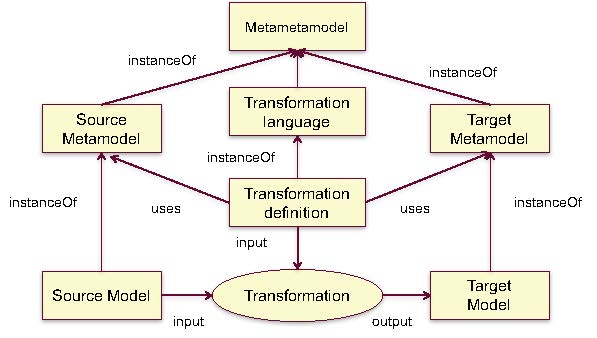
\includegraphics[scale=0.39]{PastedGraphic-1}
\caption{Transformations in model-driven engineering}
\label{fig:PastedGraphic-1}
\end{figure}

The set of mappings from SSN to SAREF is a transformation definition, which is an instance of a transformation language. For the implementation of these mappings, a transformation language could be the library Apache JENA\footnote{\url{https://jena.apache.org/}} (Java) and the mappings (transformation definition), which uses the SSN (source) and SAREF (target) metamodels, an instance of JENA implementation. The mappings and a message according to SSN (source) are used as input by the transformation runtime executor, e.g. Java Runtime Environment (JRE), which produces a SAREF (target) ontology with similar semantics of the original. 

We use a specification strategy to avoid conceptual errors during the implementation, which is a common issue in software engineering. Moreover, directly implementing the mappings forces a preliminary choice of the technology of the transformation runtime, which means coupling the mappings with a technology, i.e. limiting the reuse of the mappings. Our ontology-driven conceptual modeling strategy \cite{Moreira2017} can address this issue by leveraging the MDE approach with a specification artifact targeted to human readers, i.e. the transformation developers. For specification, the transformation runtime executor is not considered. Instead of a formal language for the transformation definition it is used a natural language or a pseudo-code approach, similar to the OASIS EDXL-TEP and HL7 (syntactic interoperability standards) transformations \footnote{\url{http://docs.oasis-open.org/emergency/TEP-HL7v2-transforms/v1.0/TEP-HL7v2-transforms-v1.0.html}}. 

This approach enables to (re)use the specification for different strategies of ontology alignments’ implementation. The implementation of our mappings, i.e. the transformation definition, will be developed through configuration files (XML) as an instance of the IPSM configuration schema (transformation language). However, this is an ongoing activity and this paper only covers the specification artifact, presented through pseudo-code approach in section 4. Therefore, we produced an initial documentation regarding the classes and object properties of both ontologies and their possible relations, analyzing each class/object property according to the definitions. In particular, the DUL ontology used by SSN also supported our ontological analysis of the terms and their intended concepts, serving as foundations for the main classes, e.g. \textit{ssn:\-SensingDevice} is a \textit{DUL:PhysicalObject} and a \textit{DUL:\-Designed\-Artifact}.

A common approach after specifying (before implementing) is to evaluate whether the mappings will produce the correct ontology (output) from the inputted ontology, i.e. if an ontology according to SAREF can be produced by the SSN to SAREF mappings' specification. As an initial evaluation of this specification, we simulate an unidirectional semantic translation from WM30 ontology, represented as an extension of SSN, to an ontology represented as SAREF. In general, the result from the translations must represent the WM30 wind sensor with SAREF, keeping similar semantics of the original. Therefore, the goal of this evaluation is to check the semantic similarity between the original and the final ontologies. Here we used an approach based on competency questions to measure this similarity. A list of competency questions is presented and each question is responded by querying the elements (classes, properties and instances) of both ontologies. The responses are compared to verify whether the semantics is maintained after executing the translation. Intentionally, the competency questions were conceived according to the expressiveness of the SSN WM30 ontology, targeting its main elements, as the different measurement capabilities described in the technical specifications\footnote{\url{http://www.vaisala.fi/Vaisala\%20Documents/Brochures\%20and\%20Datasheets/WM30-Datasheet-B210384EN-B-LoRes.pdf}}. For example, the accuracy of the WM30 wind speed sensor (within a range from 0.4 to 60 m/s) is +- 0.3 m/s for wind speed less than 10 m/s and +-2\% of variance for wind speed grater than 10 m/s. For each question, at first we answered the question based on the original ontology (in SSN) and, then, we answered the same question for the generated ontology (SAREF). Second, we compare whether the semantics of the response is similar to each other, i.e. if the semantics is lost or maintained. 

Competency questions: 
\\\textbf{CQ01.} What are the main characteristics of the Vaisala WM30 sensor? 
\\\textbf{CQ02.} What is the composition of this sensor, i.e. what other devices are part of WM30?
\\\textbf{CQ03.} What measurement properties this sensor provides?
\\\textbf{CQ04.} What are the accuracy, delay distance, starting threshold and damping ratio of WMS30 wind direction sensors? 
\\\textbf{CQ05.} What measurement range constraints differentiate these types of wind direction sensors?
%\\CQ06. What are the distance constant, starting threshold and transducer output of wind speed sensors? 
%\\CQ07. What are the ranges of accuracy and condition ranges  constraints differentiate these types of wind speed sensors?
%\\CQ08. What is the characteristic transfer function of WM30?



%%%%%%%%%%%%%%%%%%% SEC: SEMANTIC TRANSLATIONS %%%%%%%%%%%%%%%%%%% 

\section{SEMANTIC TRANSLATIONS}

\subsection{Mappings: SSN to SAREF}

\begin{figure}[h!]
\centering
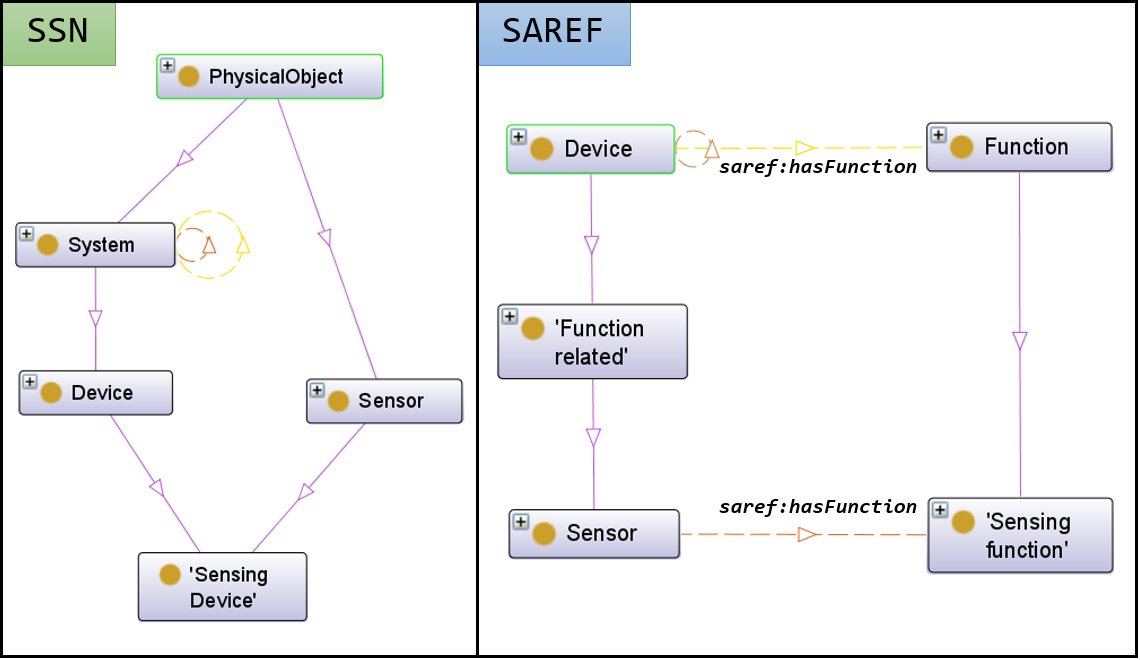
\includegraphics[scale=0.28]{SSN_SAREF_SensingDevice_Device}
\caption{Main elements of SSN and SAREF}
\label{fig:SSN_SAREF_SensingDevice_Device}
\end{figure}

Mappings between SSN and SAREF were specified through an ontological analysis of their TBox, i.e. concepts and roles definitions (predicates) with logical operations. A study was made on how SSN and SAREF describe the characteristics of sensors, including their capabilities of observation. The mappings follow a logic sequence according to the main elements and similar structures of SSN and SAREF. 

Here we detail only the mappings from SSN to SAREF because of space limitation, the other direction (from SAREF to SSN) will be reported in the future. For each mapping a code snippet is presented, as a pseudocode, to illustrate the creation of the ontology using SAREF. While the main element in SSN is the \textit{Sensing Device}, which is a subclass of \textit{Device} and \textit{Sensor}, in SAREF the main element is \textit{Device}, which can be specialized as a \textit{Sensor} related to \textit{Sensing Function}. 

\subsubsection{M01. ssn:\-SensingDevice -> saref:\-Sensor}
The characteristics of \textit{ssn:\-SensingDevice}, inherited from \textit{ssn:\-Sensor} and \textit{ssn:\-System}, is mapped to \textit{saref:\-Sensor}, which inherits \textit{saref:\-Device} properties, including the relationship with the \textit{saref:\-SensingFunction} (\textit{saref:\-hasFunction}). The code snippet below illustrates this mapping. 

\begin{lstlisting}[caption={Pseudocode snippet for M01},label={code:sample}]
IN: {ssn_sensingDevice}  
create saref_sensor = saref:Sensor  
saref_sensor.rdfs = ssn_sensingDevice.rdfs    
create saref_function = saref:SensingFunction  
create saref_hasFunction = saref:hasFunction  
create saref_sensor saref_hasFunction saref_function  

\end{lstlisting}

Figure \ref{fig:SSN_SAREF_SensingDevice_Device} illustrates the elements involved in this mapping. Notice that, indirectly, this mapping also transforms from \textit{ssn:\-Sensor} to \textit{saref:\-Sensor}.

\subsubsection{M02. ssn:\-hasSubSystem -> saref:\-consistsOf}

\begin{lstlisting}[caption={Pseudocode snippet for M02},label={code:sample}]
IN: {ssn_sensingDevice, saref_sensor}
for each ssn_system in ssn_sensingDevice.ssn:hasSubSystem 
  create saref_device_component = saref:Device 
  
  if ssn_system is ssn:SensingDevice then
    saref_device_component = Map(M01, ssn_system) 
  else if ssn_system is ssn:Device then 
    saref_device_component.rdfs = ssn_system.rdfs 
   
  create saref_consistsOf = saref:consistsOf 
  create saref_sensor saref_consistsOf saref_device_component 
end for
\end{lstlisting}

Once executing M01, the next step is to check the composition relationship of a device, i.e. the components that are part of a device, which are characterized by both SSN and SAREF. In SSN, the object property \textit{ssn:\-hasSubSystem} relating two \textit{ssn:\-System} represents this relationship. In SAREF, the object property \textit{saref:\-consistsOf} plays this role, relating two \textit{saref:\-Device} in a similar way, both illustrated in Figure \ref{fig:SSN_SAREF_SensingDevice_Device} as a self-relationship. Therefore, when \textit{ssn:\-hasSubSystem} is used between the \textit{ssn\_sensingDevice} (from M01) and a \textit{ssn:\-System}, which must be a \textit{ssn:\-Device} or a \textit{ssn:\-SensingDevice}, then it is mapped to \textit{saref:\-consistsOf} object property of the \textit{saref\_sensor} (created in M01). If the device component is a \textit{ssn:\-SensingDevice}, then a recursive algorithm is used by applying M01 to it. If the device component is a \textit{ssn:\-Device}, then it is created a \textit{saref:\-Device}. The code snippet below illustrates this mapping.

\subsubsection{M03. ssn:\-observes -> saref:\-measuresProperty}
Once executing M01 and M02, the next step is to map the measurement property which the sensor is able to observe, i.e. the measurement property of a sensor. For example, a wind sensor is able to observe both wind direction and wind speed. Therefore, the \textit{ssn:\-observes} of a \textit{ssn:\-SensingDevice} is mapped to \textit{saref:\-measuresProperty} of a \textit{saref:\-Device}. These object properties relate to \textit{ssn:\-Property} and \textit{saref:\-Property}, respectively. Therefore, this mapping also includes the creation, if it does not exist, of the \textit{ssn:\-Property}. At last, this mapping needs to create the relationship back from the \textit{saref:\-Property} to the \textit{saref:\-Device} through the object property \textit{saref:\-isMeasuredByDevice}. The code snippet below illustrates this mapping. 

\begin{lstlisting}[caption={Pseudocode snippet for M03},label={code:sample}]
IN: {ssn_sensingDevice, saref_sensor}
for each p in ssn_sensingDevice.observes 
  create ssn_property = p
  create saref_property = saref:Property 
  saref_property = GetPropertyInSAREF(ssn_property)
    
  if not isnull(saref_property) then 
    saref_property.rdfs = ssn_property.rdfs 
 
  create saref_measuresProperty = saref:measuresProperty 
  create saref_sensor saref_measuresProperty saref_property 
  create saref_isMeasuredByDevice = saref:isMeasuredByDevice
  create saref_property saref_isMeasuredByDevice saref_sensor
end for
\end{lstlisting}

\subsection{Evaluation}
As described in the methodology section, an execution of the mappings presented above was simulated having the WM30 wind sensor example (according to SSN) as input. The output of this translation, i.e. the WM30 ontology according to SAREF (in TTL) was produced and made available (\url{https://github.com/jonimoreira/SSN-SAREF}). The answers of the competency questions, listed in methodology section, were produced by navigating and querying (SPARQL) this generated ontology with support of an ontology editor (Protegé (\url{http://protege.stanford.edu}) and TopBraid Composer(\url{http://www.topquadrant.com/products})). The competency questions were responded as follows:
%%%%%%%%%%%%%%%%%%%%%%%%%%%%%%%%%%%%%%%%%%%%%%%%%%%%%%%%%%%%%%%%%%%%%%%%%%%%%%%%%
\\\\\textbf{CQ01.} In the original ontology (SSN), the main characteristics of the Vaisala WM30 sensor can be extracted by starting the navigation in the \textit{WM30:\-Vaisala\-\_WM30} element, which is a \textit{ssn:\-SensingDevice}, inheriting the properties from \textit{ssn:\-Device} and \textit{ssn:\-Sensor}. Besides, the \textit{rdfs:comment} with a general description of this wind sensor, it represents that the sensor is composed by two sensors (\textit{WM30:\-WM30\-\_Wind\-Direction} and \textit{WM30:\-WM30\-\_WindSpeed)}, one for wind direction and another for wind speed (both \textit{ssn:\-Sensor}). Moreover, WM30 sensor can measure (observe) the types (properties) \textit{WM30:\-WindDirection} and \textit{WM30:\-WindSpeed} (both \textit{ssn:\-Property}). Figure \ref{fig:SSN_SystemProperties} illustrates these properties.

\begin{figure}[h!]
\centering
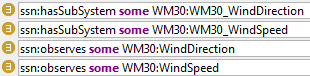
\includegraphics[scale=0.98]{SSN_SystemProperties}
\caption{Vaisala WM30 \textit{Sensing Device}} (SSN)
\label{fig:SSN_SystemProperties}
\end{figure}

In the generated ontology (SAREF), according to M01, \textit{WM30:\-Vaisala\-\_WM30} element is created as a \textit{saref:\-Sensor}. A \textit{saref:\-SensingFunction} is created and the \textit{WM30:\-Vaisala\-\_WM30} element linked to it through \textit{saref:\-hasFunction} property. According to M02, the composition of the sensor \textit{WM30:\-Vaisala\-\_WM30} is derived from the \textit{ssn:\-hasSubSystem} properties, i.e. \textit{WM30:\-WM30\-\_Wind\-Direction} and \textit{WM30:\-WM30\-\_WindSpeed}, as depict in Figure \ref{fig:SSN_SystemProperties}. M03 produced the measurement properties of the sensor from the \textit{ssn:\-observes element}, i.e. \textit{saref:\-measuresProperty} to \textit{WM30:\-WindDirection} and \textit{WM30:\-WindSpeed}. Figure \ref{fig:SAREF_Sensor_WM30} illustrates the result \textit{WM30:\-Vaisala\-\_WM30)} as a \textit{saref:\-Sensor}. Therefore, by navigating to \textit{WM30:\-Vaisala\-\_WM30}, a \textit{saref:\-Sensor}, it is possible to respond this competency question in a similar way from the original, i.e. the semantics is completely maintained.  
\begin{figure}[h!]
\centering
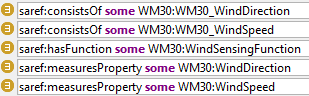
\includegraphics[scale=0.98]{SAREF_Sensor_WM30}
\caption{Vaisala WM30 \textit{Sensing Device} (SAREF)}
\label{fig:SAREF_Sensor_WM30}
\end{figure}
\\\textbf{CQ02.} In the original ontology (SSN), the composition of Vaisala WM30 sensor can be extracted by navigating from the \textit{WM30:\-Vaisala\-\_WM30} element to the \textit{ssn:\-hasSubSystem} properties, i.e. \textit{WM30:\-WM30\-\_Wind\-Direction} and \textit{WM30:\-WM30\-\_WindSpeed}, both \textit{ssn:\-Sensor}. In particular, the WM30 wind direction sensor (\textit{WM30:\-WM30\-\_Wind\-Direction}) can have one wiper (\textit{WM30:\-WMS301}) or two (\textit{WM30:\-WMS302}), which has greater measurement range. The same structure is generated in SAREF, resulted from M02, having \textit{WM30:\-WM30\-\_Wind\-Direction} and \textit{WM30:\-WM30\-\_WindSpeed} created as \textit{saref:\-Device}, linked through the object property \textit{saref:\-consistsOf}. It is possible to achieve the same structure of \textit{WM30:\-WM30\-\_Wind\-Direction} and \textit{WM30:\-WM30\-\_WindSpeed}, including the specialization to one or two wipers, by navigating from \textit{WM30:\-Vaisala\-\_WM30} (\textit{saref:\-Sensor}) through \textit{saref:\-consistsOf}. Therefore, this competency question is responded in a similar way from the original, i.e. the semantics is completely maintained.
%%%%%%%%%%%%%%%%%%%%%%%%%%%%%%%%%%%%%%%%%%%%%%%%%%%%%%%%%%%%%%%%%%%%%%%%%%%%%%%%%
\\\\\textbf{CQ03.} In the original ontology (SSN), the measurement properties of Vaisala WM30 sensor can be extracted by navigating from the \textit{WM30:\-Vaisala\-\_WM30} element through the \textit{ssn:\-observes} properties, i.e. \textit{WM30:\-WindDirection} and \textit{WM30:\-WindSpeed}, both \textit{ssn:\-Property}. WM30 original example also uses an ontology of Quantity Kinds (\url{http://purl.oclc.org/NET/ssnx/qu}) through the element \textit{qu:QuantityKind} as \textit{ssn:\-Property}. This element provides a taxonomy of quality dimensions, making use of \textit{dim:Angle} for \textit{WM30:\-WindDirection} and \textit{dim:VelocityOrSpeed} for \textit{WM30:\-WindSpeed}. The same structure is generated in SAREF, resulted from M03, as \textit{saref:\-Property}. Therefore, similar to CQ01 and CQ02, the semantics is completely maintained.
%%%%%%%%%%%%%%%%%%%%%%%%%%%%%%%%%%%%%%%%%%%%%%%%%%%%%%%%%%%%%%%%%%%%%%%%%%%%%%%%%
\\\\\textbf{CQ04.} The specification of the WMS30 wind direction sensor (Figure \ref{fig:WM30specifications}) describes the accuracy, delay distance, starting threshold and damping ratio of this sensor. For example, accuracy can vary from -3 to 3 degrees, while the delay distance is 0.6 meters and the starting threshold is lower than 1.0 m/s.  
In the original ontology (SSN), the measurement capabilities of each wind direction and speed components  of Vaisala WM30 sensor can be extracted by navigating from the \textit{WM30:\-Vaisala\-\_WM30} element through the \textit{ssn:\-hasSubSystem} properties, i.e. \textit{WM30:\-WM30\-\_Wind\-Direction} and \textit{WM30:\-WM30\-\_WindSpeed}, both \textit{ssn:\-Sensor}, as described in CQ02. The WM30 wind direction sensor with one wiper (\textit{WM30:\-WMS301}) has measurement capability a  \textit{WM30:\-WM30\-\_Wind\-Direction\-\_MeasurementCapability\-\_WMS301} (similar for \textit{WM30:\-WMS302}). A \textit{WM30:\-WM30\-\_Wind\-Direction\-\_MeasurementCapability\-\_WMS301} is a \textit{WM30:\-WM30\-\_Wind\-Direction\-\_MeasurementCapability}, which describes the ranges supported (restrictions) for accuracy, delay distance, starting threshold and damping ratio, illustrated in the axioms of Figure \ref{fig:SSN_MeasurementCapability}. \textit{ssn:\-MeasurementCapability} is a \textit{ssn:\-Property}.
Notice that, regarding the accuracy, SSN provides naively the \textit{ssn:\-Accuracy} element which can be used to extract the accuracy of all involved sensors through a simple SPARQL query (SELECT * WHERE \{ ?a ?b ssn:\-Accuracy. \}) .  
\begin{figure}[h!]
\centering
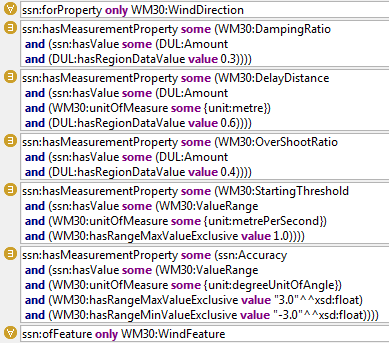
\includegraphics[scale=0.87]{SSN_MeasurementCapability}
\caption{Wind direction measurement capabilities} 
\label{fig:SSN_MeasurementCapability}
\end{figure}

In the generated ontology (SAREF), these measurement capabilities were lost because there is not a similar structure of \textit{ssn:\-MeasurementCapability} in SAREF, thus, no mappings were added to consider the  \textit{ssn:\-hasMeasurementCapability} object property of \textit{ssn:\-Sensor}. Therefore, this question could not be responded with the generated ontology (semantics was lost).  
\\\\\textbf{CQ05.} In the original ontology (SSN), the measurement range constraints differentiating 301 and 302 wind direction sensors can be extracted by analyzing the restrictions of \textit{WM30:\-WM30\-\_Wind\-Direction\-\_Measurement\-Capability\-\_WMS\-301} and \textit{WM30:\-WM30\-\_Wind\-Direction\-\_Measurement\-Capability\-\_WMS\-302} regarding the object property \textit{ssn:\-has\-Measurement\-Property}. The first restricts the measurement range from 0 to 355 degrees, while the second restricts from 0 to 360 degrees. This question could not be responded with the generated ontology because of the same reason described in CQ04, i.e. the absence of \textit{ssn:\-MeasurementCapability} in SAREF and no mappings on the \textit{ssn:\-hasMeasurementCapability} object property.


%%%%%%%%%%%%%%%%%%% SEC: DISCUSSION %%%%%%%%%%%%%%%%%%% 
\subsection{Discussion}

The evaluation above demonstrated that from 5 competency questions only 3 (60\%) could be answered with the mappings described in this paper. The main issue identified is the lack of a naive element in SAREF to describe the measurement capabilities of a sensor, which SSN enables through the \textit{ssn:\-hasMeasurementCapability} object property of \textit{ssn:\-Sensor}. To cope with this issue we suggest that a new mapping is created to import the structure from SSN, i.e. extend SAREF with the object property \textit{ssn:\-has\-Measurement\-Capability}, which will be an object property of \textit{saref:\-Sensor}. In addition, the mapping must consider to import, as a \textit{saref:\-Property}, both \textit{ssn:\-Measurement\-Capability} and \textit{ssn:\-Measurement\-Property}. This would enable the link of a \textit{saref:\-Sensor} to the \textit{ssn:\-Measurement\-Capability}, which incorporates the links to the \textit{ssn:\-Measurement\-Property}. 

A conceptual issue in SSN was identified regarding the element \textit{ssn:\-Sensor}. The description of this element states that it “allows sensors, methods, instruments, systems, algorithms and process chains as the process used of an observation (…) they are all grouped under the term sensor”. Thus, the description includes that a \textit{ssn:\-Sensor} can be a "system", but \textit{ssn:\-Sensor} was not implemented as a specialization of \textit{ssn:\-System}. In this way, \textit{ssn:\-Sensor} could also inherit the composition relationship (\textit{ssn:\-hasSubSystem}) and, thus, can represent a set of sensors. 

One issue identified in WM30 ontology regards the \textit{WM30:\-Vaisala\-\_WM30} composition of wind direction (\textit{WM30:\-WM30\-\_Wind\-Direction}) and speed (\textit{WM30:\-WM30\-\_WindSpeed}) sensors. Both are \textit{ssn:\-Sensor}, but the composition relationship (\textit{ssn:\-hasSubSystem}) is applied from a \textit{ssn:\-System} to a \textit{ssn:\-System}. Since \textit{ssn:\-Sensor} is not a \textit{ssn:\-System}, thus the mapping M02 should consider not only \textit{ssn:\-System} within \textit{ssn:\-hasSubSystem} property in the for loop. 

A practical issue when mapping to SAREF is to consider extending the taxonomy of sensor "types" by creating a new element when the type does not exist in SAREF. For example, smoke and temperature sensors are classified as \textit{saref:\-SmokeSensor} and \textit{saref:\-TemperatureSensor,} respectively, having  function (\textit{saref:\-hasFunction}) and measure property (\textit{saref:\-measuresProperty}), linking the type of the sensor with functions it has and the type of property it measures (\textit{saref:\-Smoke} and \textit{saref:\-Temperature}. Thus, in our example, the correct implementation for the wind sensor is to create the subclass \textit{saref:\-WindSensor}, with function sensing and measuring the properties of wind direction and wind speed, which is guaranteed by M01. 


%%%%%%%%%%%%%%%%%%% SEC: CONCLUSIONS %%%%%%%%%%%%%%%%%%% 
\section{CONCLUSIONS}

In this paper we described the initial mappings between SSN and SAREF towards their ontological alignments to enable the semantic integration of IoT platforms relying on them. In particular, the mappings presented here focused in translating the main parts of a sensor ontology, i.e. the elements about sensor, device, its composition and functions. Here we detailed three mappings to cover these properties, showing how to produce a SAREF ontology from a SSN ontology through a semantic translation mechanism. An evaluation was performed to validate the initial specification produced, which used an ontology of wind sensor with SSN (WM30, provided by W3C) as input and generates a SAREF-based ontology as output. The results demonstrated a coverage of 60\% of semantics maintained from the original ontology (SSN) to the generated (SAREF). 

The main issue identified is the lack of measurement capabilities in SAREF to represent the collection of measurement properties of a component of a sensor. For example, the wind direction component of the WM30 wind sensor measures the wind direction property, which has a specific configuration of accuracy, delay distance, starting threshold and damping ratio. Therefore, we identified that the representation of these characteristics in SAREF needs to be addressed, probably by extending it with the \textit{ssn:\-has\-Measurement\-Capability} object property (used by \textit{saref:\-Sensor}) and importing \textit{ssn:\-Measurement\-Capability} and \textit{ssn:\-Measurement\-Property} (as \textit{saref:\-Property}).

From this initial iteration on the development of the bi-directional semantic translations we can conclude that, although the mappings presented here are quite intuitive, they reflect the foundations of the ontology alignments between SSN and SAREF and is a required first step towards complete semantic translations between them. Therefore, it represents a relevant contribution to the state-of-art by enabling a basic level of semantic interoperability between IoT platforms relying on SSN and SAREF. 

Future work includes the acquisition and/or generation of test datasets (in both SSN and SAREF), giving emphasis to the requirements for an early warning system \cite{Moreira2017} to detect accidents in the port of Valencia, an INTER-IoT application scenario. New mappings will be created according to this scope with incremental evaluations, using the test datasets to verify whether the semantic interoperability is improved or not. Then, these mappings will be implemented through configurations in IPSM, exposing semantic translation services that will be consumed by the early warning system. 


%ACKNOWLEDGMENTS are optional
\section{Acknowledgments}
Thanks for the Brazilian funding agency (CAPES, BEX 1046/14-4) and EU-H2020-ICT grant INTER-IoT 687283.

%
% The following two commands are all you need in the
% initial runs of your .tex file to
% produce the bibliography for the citations in your paper.
\bibliographystyle{abbrv}
\bibliography{Semantics2017_references}  % sigproc.bib is the name of the Bibliography in this case
% You must have a proper ".bib" file
%  and remember to run:
% latex bibtex latex latex
% to resolve all references
%
% ACM needs 'a single self-contained file'!
%
%APPENDICES are optional
%\balancecolumns




\end{document}
